\begin{justify}
    \subsection{Analyse et critique des applications similaires}
    L’analyse des applications concurrentes permet d’identifier les axes d’amélioration, afin d’optimiser notre solution et de concevoir une expérience utilisateur répondant aux attentes du marché.
    \subsubsection{Outils d’automatisation des tests de pénétration\cite{etdeExistant}}
        Un scanner de vulnérabilités analyse un site web afin de détecter les risques liés au code source et aux liens en identifiant des menaces telles que les malwares, les injections SQL, les failles XSS. Le choix d’un outil dépend de plusieurs critères: la complexité du site, la couverture des vulnérabilités, la qualité des rapports générés et la capacité à effectuer des analyses régulières\cite{etdeExistant}.

        Nous avons sélectionné les outils suivants comme solutions similaires à notre application dans la partie dédiée aux tests de pénétration, afin d’en analyser les fonctionnalités et les limites.
        \begin{enumerate}[label=\alph*)]
            \item \textbf{HostedScan\cite{etdeExistant}:} est un service en ligne basé sur des scanners 100\% open-source, il automatise la détection des vulnérabilités sur les réseaux, serveurs et applications web. Il centralise la gestion des failles, facilite la priorisation des tâches, la génération de rapports, et renforce la sécurité de leurs clients. Ce service inclut plusieurs types de scanners:  
            \begin{itemize}[label=$\bullet$]
                    \item \textbf{Des vulnérabilités réseau}: identifie les \acs{CVE} et les logiciels obsolètes.  
                    \item \textbf{Des applications web}: détecte les injections SQL, les bibliothèques JavaScript vulnérables, les scripts intersites (\acs{XSS}) et autres menaces.  
                    \item \textbf{Des ports TCP/UDP}: repère les erreurs de configuration des pare-feu et du réseau.  
                    \item \textbf{TLS/SSL}: valide les certificats et recherche les vulnérabilités Heartbleed et Robot.  
                \end{itemize}
                
            La Figure~\ref{fig:Hostedscan} présente l’interface du tableau de bord de l’application HostedScan, illustrant les résultats des analyses ainsi que les principales fonctionnalités proposées.
                \begin{figure}[H]
                    \centering
                   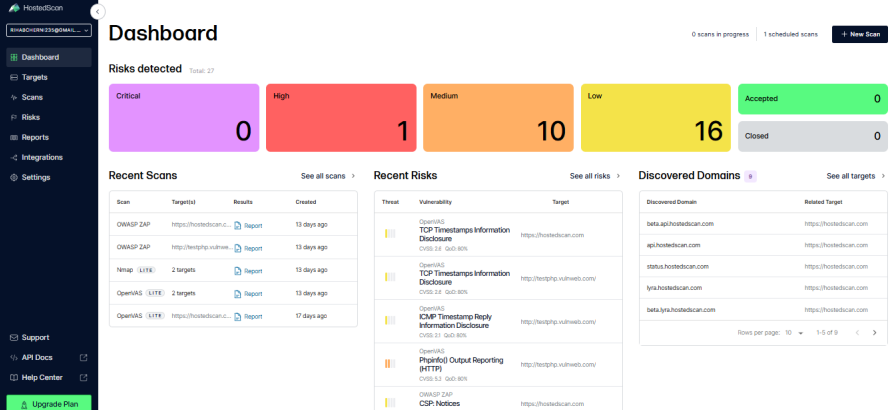
\includegraphics[width=\textwidth]{chapitres/ch1/img/existant/hostedscan.PNG}
                    \caption{Interface du l’application Hostedscan\cite{hostedscanimg}}
                    \label{fig:Hostedscan}
                \end{figure}
            \vspace{-0.1cm}
            \item \textbf{Invicti\cite{invicti} :} est un outil de sécurité web avancé permettant de protéger les applications, services web et API contre une large gamme de vulnérabilités, telles que les injections SQL, les failles \acs{XSS} et les erreurs de configuration SSL/TLS. Il réalise également des tests de configuration des serveurs web et se distingue par son moteur d’analyse basé sur la preuve, qui confirme automatiquement l’exploitabilité des failles détectées, réduisant ainsi les faux positifs. Son moteur d’exploration intelligent est compatible avec les technologies dynamiques modernes (JavaScript, Ajax, React, Angular), ce qui le rend efficace pour l’analyse des applications complexes.\\Invicti s’intègre facilement aux pipelines DevOps et CI/CD, favorisant une automatisation continue de la sécurité. Il propose en outre des tableaux de bord interactifs, des rapports personnalisables et des fonctionnalités de gestion des vulnérabilités, facilitant la collaboration entre les développeurs et les équipes de sécurité.
            
            La Figure~\ref{fig:Invicti} montre l’interface de l’outil Invicti, mettant en évidence les résultats d’analyse de sécurité web ainsi que les fonctionnalités de gestion des vulnérabilités.
            \begin{figure}[H]
                \centering
               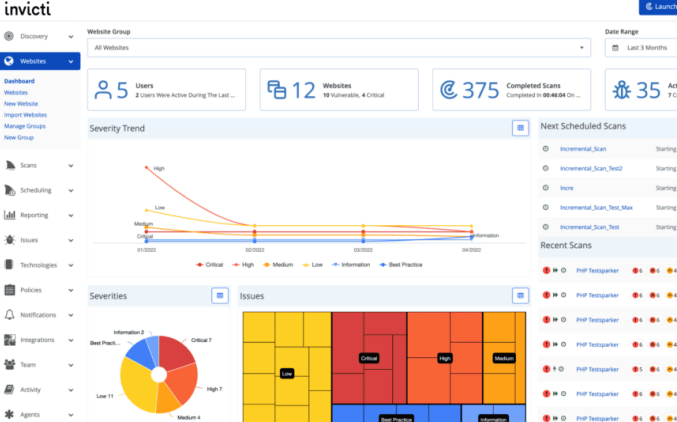
\includegraphics[width=\textwidth]{chapitres/ch1/img/existant/invicti.png}
                \caption{Interface du l’application Invicti\cite{invicti}}
                \label{fig:Invicti}
            \end{figure}
            \vspace*{-0.4cm}
        \end{enumerate}
    \subsubsection{Outils d’automatisation des tests fonctionnels:}
        L’automatisation des tests fonctionnels est essentiel pour assurer la qualité et la fiabilité des applications. Plusieurs outils sont disponibles qui offrent des fonctionnalités variées comme:
        \begin{enumerate}[label=\alph*)]
           \item  \textbf{Cypress}\cite{Cypress} est un outil d'automatisation de tests fonctionnels pour les applications web, apprécié pour sa rapidité, sa fiabilité et sa simplicité d'utilisation. Il permet d’automatiser des tests de composants, d’API et d’accessibilité, tout en assurant la compatibilité multi-navigateurs. Grâce à son interface de débogage en temps réel, son exécution locale rapide et sa facilité d’intégration, il constitue une solution complète pour les tests web.

           La Figure~\ref{fig:Cypress} illustre l’environnement de test automatisé proposé par Cypress, affichant les scénarios exécutés, les résultats des tests, et les options de débogage.
                \begin{figure}[H]
                \centering
               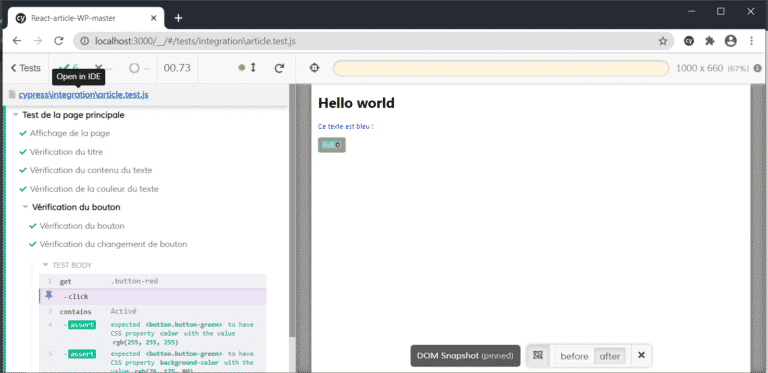
\includegraphics[width=\textwidth]{chapitres/ch1/img/existant/cpress.PNG}
               \caption{Interface de démonstration de Cypress exécutant une suite de tests \cite{imgCypress}}
                \label{fig:Cypress}
            \end{figure}
                \vspace{-0.4cm}
            \item  \textbf{Katalon Studio\cite{Katalon}:} est un outil d'automatisation des tests pour les applications web et mobiles, basé sur Selenium. Il offre une interface conviviale permettant de créer et d’exécuter des tests sans compétences techniques avancées. Son intégration avec des outils comme Jira et Slack, ainsi que son support des tests continus et du suivi instantané des résultats, en fait une solution efficace pour assurer la qualité tout au long du développement.

            La Figure~\ref{fig:Katalon-Studio} présente l’interface de Katalon Studio, illustrant l’organisation des cas de test ainsi que le suivi de leur exécution.
            \begin{figure}[H]
                \centering
                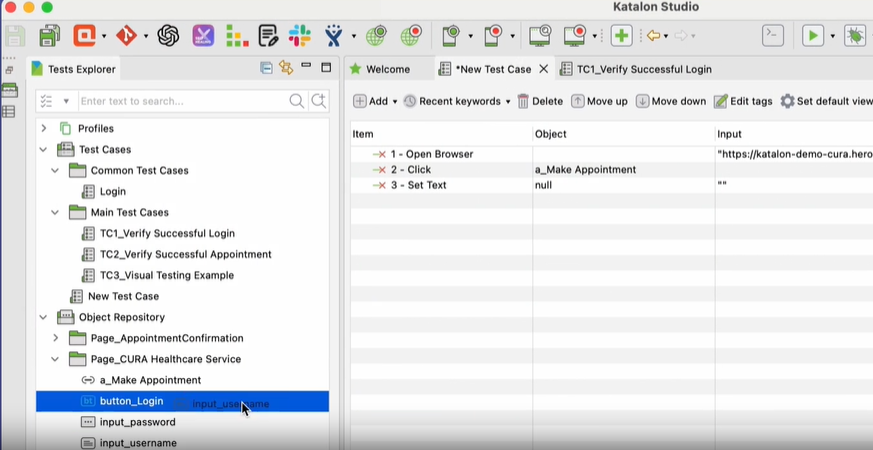
\includegraphics[width=\textwidth]{chapitres/ch1/img/existant/katal.PNG}
                \caption{Interface du l’application Katalon Studio\cite{Katalon}}
                \label{fig:Katalon-Studio}
            \end{figure}
            \vspace{-0.3cm}
    \end{enumerate}
    
    \subsubsection{Outils d’automatisation des tests SEO}
        Le \textbf{SEO (Search Engine Optimization)} est indispensable pour renforcer la visibilité d’un site sur les moteurs de recherche.Il permet d’identifier les erreurs, d’optimiser les performances et de vérifier le respect des bonnes pratiques. Plusieurs outils automatisent ces audits en analysant les mots-clés, le contenu, les aspects techniques, le positionnement, et en générant des recommandations et des rapports. Voici une analyse des plus pertinents.  
        \begin{enumerate}[label=\alph*)]
            \item \textbf{Semrush\cite{seoTools}:} est un outil SEO les plus populaires et complets du marché. Il propose une large gamme de fonctionnalités: l’analyse de mots-clés, l’audit technique, la veille concurrentielle, le suivi de positionnement, la gestion des backlinks, l’analyse du temps moyen passé sur le site ainsi que l’identification des pages les plus performantes. Son outil de suivi de positionnement fournit des analyses précises et évolutives, permettant aux professionnels du marketing digital de surveiller efficacement la performance de leurs mots-clés sur les moteurs de recherche. Il permet également de réaliser des audits SEO détaillés et de générer des rapports visuels pour le suivi des performances dans le temps.

            La Figure~\ref{fig:Semrush} illustre le tableau de bord de SEMrush, mettant en évidence les résultats de l’audit SEO ainsi que les performances globales du site web.
            \begin{figure}[H]
                \centering
                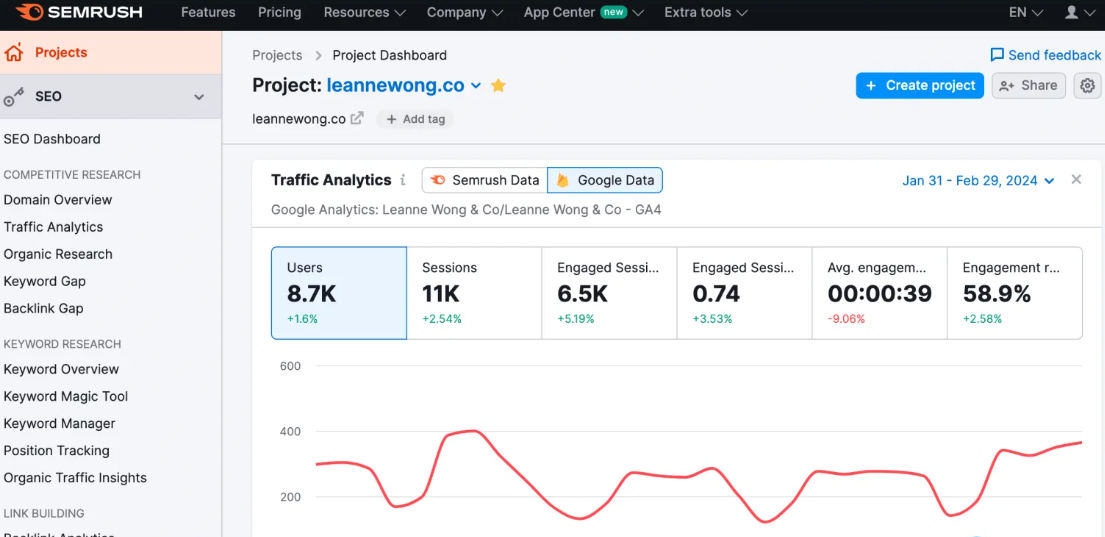
\includegraphics[width=\textwidth]{chapitres/ch1/img/existant/semrush.PNG}
                \caption{Interface de l’outil Semrush\cite{seoTools}}
                \label{fig:Semrush}
            \end{figure}
        \vspace{-0.3cm}
        \item \textbf{Ahrefs\cite{seoTools}} est une plateforme SEO reconnue pour la puissance de sa base de données de backlinks et ses capacités avancées d’analyse concurrentielle. Elle permet d’ajuster efficacement sa stratégie de contenu en observant les performances des concurrents sur les moteurs de recherche. L’outil offre des fonctionnalités telles que le suivi du positionnement des mots-clés, l’identification des pages les plus génératrices de trafic, l’analyse des liens entrants et l’accès à l’historique du positionnement via des visualisations graphiques.

        La Figure~\ref{fig:AhrefsAudit} présente l’interface d’Ahrefs, mettant en évidence le suivi du positionnement ainsi que les principaux indicateurs de performance SEO.
            \begin{figure}[H]
                \centering
                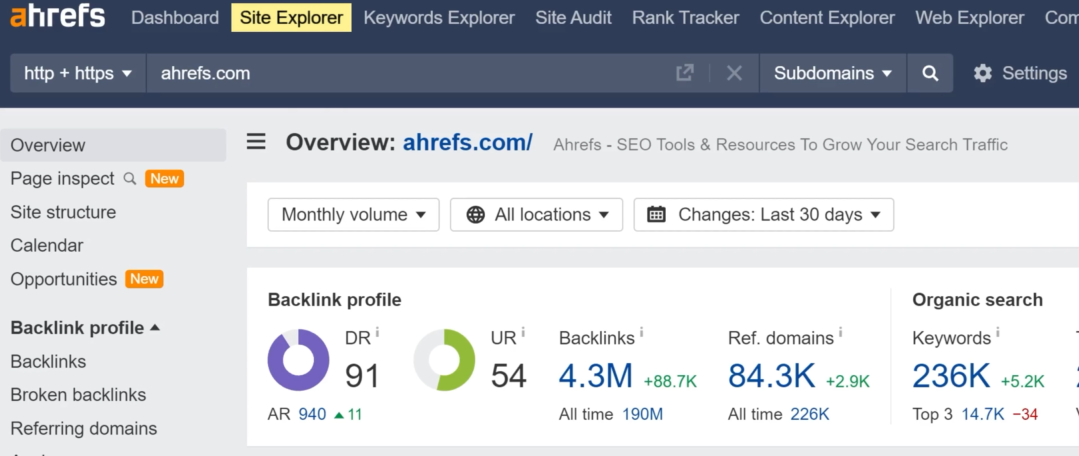
\includegraphics[width=\textwidth]{chapitres/ch1/img/existant/ahrefs.PNG}
                \caption{Interface de l’outil Ahrefs Site Audit\cite{seoTools}}
                \label{fig:AhrefsAudit}
            \end{figure}
            \vspace{-0.3cm}
        \end{enumerate}    
    \subsubsection{Critique de l’existant:}
        Le tableau ~\ref{tab: comparaison} présente une  comparaison détaillée des principaux outils analysés précédemment.
        \begin{spacing}{1.5}
            \begin{longtable}{|p{2.7cm}|p{6.6cm}|p{6.6cm}|}
                \caption{\centering Tableau comparatif des outils d’automatisation}
                \label{tab: comparaison}\\ \hline
                         \multicolumn{3}{|c|}{\textbf{Outils d’automatisation des tests de pénétration \cite{etdeExistant}}} \\
                        \hline
                        \textbf{Application} & \textbf{HostedScan} & \textbf{Invicti}\\
                        \hline
                            \textbf{Score}\footnote{Le score Geekflare est attribué par une équipe éditoriale selon plusieurs critères techniques et fonctionnels (source : \href{https://geekflare.com/fr/cybersecurity/best-website-security-scanner/}{Geekflare}).}& 
                                4.2/5 &
                                4.5/5
                                \\  \hline
                             \begin{minipage}[t]{2.8cm}
                                \textbf{Profondeur d’analyse}
                            \end{minipage}& 
                            \begin{minipage}[t]{6.6cm}
                                 \justifying Réseaux, serveurs, applications web
                            \end{minipage}
                                &
                             \begin{minipage}[t]{6.6cm}
                                 \justifying API, sites, applications, services et serveurs web.
                                 \vspace{0.2cm}
                            \end{minipage}
                            \\ 
                        \hline
                             \begin{minipage}[t]{2.9cm}
                                 \textbf{Fonctions principales}
                            \end{minipage}& 
                            \begin{minipage}[t]{6.6cm}
                                 \justifying Scanners open-source et gestion centralisée des vulnérabilités.
                            \end{minipage}
                                &
                            \begin{minipage}[t]{6.6cm}
                                 \justifying Analyse basée sur la preuve et exploitation automatique des vulnérabilités.
                                \vspace{0.2cm}
                            \end{minipage}\\ 
                        \hline
                            \textbf{Avantages} & 
                                \begin{minipage}[t]{6.6cm}
                                     \justifying
                                    \begin{itemize}[left=-0.1cm, label=\textcolor{green}{$\checkmark$}]
                                        \item Détection et notification en temps réel des menaces  
                                        \item Analyse approfondie.
                                        \item Rapports personnalisables.
                                        \item Offre un plan gratuit.  
                                    \end{itemize}
                                    \vspace{0.1cm}
                                \end{minipage}
                                &
                                \begin{minipage}[t]{6.6cm}
                                     \justifying 
                                    \begin{itemize}[left=-0.1cm, label=\textcolor{green}{$\checkmark$}]
                                        \item Excellent support client.
                                        \item Fournit des rapports et des analyses détaillés.
                                        \item Faible nombre de faux positifs.
                                    \end{itemize}
                                \end{minipage}\\ 
                            \hline
                            \textbf{Inconvénients} & 
                                \begin{minipage}[t]{6.6cm}
                                     \justifying
                                    \begin{itemize}[left=-0.1cm, label=\textcolor{red}{\ding{56}}]
                                        \item Interface utilisateur peu ergonomique  
                                         \item Limité aux scanners open-source 
                                    \end{itemize}
                                    \vspace{0.1cm}
                                \end{minipage} &
                                \begin{minipage}[t]{6.6cm}
                                     \justifying
                                    \begin{itemize}[left=-0.1cm, label=\textcolor{red}{\ding{56}}]
                                        \item Absence de tarification initiale.
                                        \item Les analyses prennent parfois beaucoup de temps
                                    \end{itemize}
                                \end{minipage}\\
                            \hline
                            \textbf{Tarification} & 
                               \begin{minipage}[t]{6.6cm}
                                     \justifying
                                    \begin{itemize}[left=-0.1cm, label=$\bullet$]
                                        \item \textbf{Gratuit}: 3 analyses par mois  
                                        \item \textbf{Basique}: 39\$ mois  
                                        \item \textbf{Premium}:109\$ mois
                                    \end{itemize}
                                    \vspace{0.1cm}
                                \end{minipage}
                                &
                                \begin{minipage}[t]{6.6cm}
                                     \justifying  Offre des prix personnalisés en fonction de vos besoins spécifiques.
                                \end{minipage}\\ 
                           \hline
    
                          \multicolumn{3}{|c|}{\textbf{Outils d’automatisation des tests fonctionnels\cite{,compTestFon2}}} \\
                        \hline
                        
                        \textbf{Application} & \textbf{Cypress} & \textbf{Katalon Studio} \\
                        \hline
                            \textbf{Score}\footnote{Le score Capterra reflète la moyenne des avis des utilisateurs sur différents critères (ergonomie, fonctionnalités, support, rapport qualité/prix)(source: \href{https://clickup.com/fr-FR/blog/228197/les-outils-de-test-d'automatisation}{ClickUp}).}
                            & 4.7/5& 4.4/5 \\ 
                        \hline
                            \begin{minipage}[t]{2.8cm}     
                                \textbf{Profondeur d’analyse}
                            \end{minipage}& 
                            \begin{minipage}[t]{6.6cm}
                                 \justifying Tests: de bout en bout, de composants, d’API, d'accessibilité.
                                 \vspace{0.1cm}
                            \end{minipage}
                                & 
                            \begin{minipage}[t]{6.6cm}
                                 \justifying Tests: UI, d'API, de charge, de performance des applications web.
                                \vspace{0.1cm}
                            \end{minipage} 
                            \\ 
                        \hline
                            \textbf{Avantages} & 
                                \begin{minipage}[t]{6.8cm}
                                    \begin{itemize}[left=-0.1cm, label=\textcolor{green}{$\checkmark$}]
                                        \item Exécution rapide, compatible multi-navigateurs.
                                        \item Facilité de configuration.
                                        \item Débogage puissant avec l'interface graphique.
                                        \item Tests fiables et résultats cohérents.
                                    \end{itemize}
                                    \vspace{0.1cm}
                                \end{minipage}
                                &
                                \begin{minipage}[t]{6.6cm}
                                     \justifying
                                    \begin{itemize}[left=-0.12cm, label=\textcolor{green}{$\checkmark$}]
                                        \item Facilité d'utilisation.
                                        \item Documentation complète et support client efficace.
                                        \item Intégration facile avec les pipelines CI/CD.
                                        \item Compatibilité multi-navigateurs et tests multiplateformes.
                                    \end{itemize}
                                    \vspace{0.1cm}
                                \end{minipage}
                                \\ 
                        \hline
                            \textbf{Inconvénients} & 
                                \begin{minipage}[t]{6.6cm}
                                     \justifying
                                    \begin{itemize}[left=-0.1cm, label=\textcolor{red}{\ding{56}}]
                                        \item Certains utilisateurs ont constaté des bugs.
                                        \item Manque d'assistance intégrée pour les tests d'applications mobiles.
                                    \end{itemize}
                                \end{minipage} &
                                \begin{minipage}[t]{6.6cm}
                                     
                                    \justifying
                                    \begin{itemize}[left=-0.1cm, label=\textcolor{red}{\ding{56}}]
                                        \item Décalage lors de l'utilisation sur certains ordinateurs portables.
                                        \item Des fonctionnalités manquantes comme l'exécution parallèle.
                                    \end{itemize}
                                    \vspace{0.1cm}
                                \end{minipage}  \\
                        \hline
                            \textbf{Tarification} & 
                               \begin{minipage}[t]{6.6cm}
                                    \begin{itemize}[left=-0.1cm, label=$\bullet$]
                                        \item \textbf{Gratuit}: Plan communautaire limité
                                        \item \textbf{Équipes}: 75\$/mois.
                                        \item \textbf{Business}: 300\$/mois
                                        \item \textbf{Entreprise}: Prix personnalisé.
                                    \end{itemize}
                                    \vspace{0.1cm}
                                \end{minipage}&
                                 \begin{minipage}[t]{6.6cm}
                                     \justifying
                                    \begin{itemize}[left=-0.15cm]
                                        \item[$\bullet$] \textbf{Gratuit}: 0\$ (Plan de base avec certaines limitations).
                                        \item[$\bullet$] \textbf{Premium}: 218\$/utilisateur/mois  
                                        \item[$\bullet$] \textbf{Entreprise}: Prix personnalisé.
                                    \end{itemize}
                                    \vspace{0.1cm}
                                \end{minipage} 
                                \\ 
                       \hline
                       \multicolumn{3}{|c|}{\textbf{Outils d’audit SEO automatisé\cite{seoTools}}} \\
                        \hline
                        \textbf{Application} & \textbf{Semrush}& \textbf{Ahrefs Site Audit} \\
                        \hline
                            \textbf{Score}\footnote{Le score Capterra correspond à la moyenne des avis utilisateurs, évaluant des critères tels que l’ergonomie, les fonctionnalités, le support et le rapport qualité/prix (sources : \href{https://www.capterra.com/p/176340/Ahrefs/}{Ahrefs} et \href{https://www.capterra.com/p/151962/SEMrush/}{SEMrush}).}
                            & 4.6/5& 4.7/5 \\ 
                        \hline 
                        \textbf{Interface utilisateur} & 
                        Simple, intuitive et rapide à utiliser & 
                        Tableaux de bord graphiques et interactifs \\
                        \hline   
                        \textbf{Fonctions principales} & 
                        Audit HTML, SEO on-page, détection de liens cassés, analyse de la vitesse, compatibilité mobile, avec export des 1résultats en PDF & Visualisation graphique, suivi des erreurs, historique des audits, recommandations, avec export des résultats sous forme de graphiques et de rapports web \\
                        \hline
                        \textbf{Avantages} & 
                       \begin{minipage}[t]{6.6cm}
                            \begin{itemize}[left=-0.15cm, label=\textcolor{green}{$\checkmark$}]
                               \item Recherche et suivi des mots-clés.
                               \item Analyse concurrentielle.
                               \item Suivi du positionnement en temps réel.
                               \item Audit technique SEO complet.
                               \item Optimisation des backlinks.
                               \item Interface personnalisable.
                             \end{itemize}
                        \end{minipage}& 
                         \begin{minipage}[t]{6.6cm}
                            \begin{itemize}[left=-0.15cm, label=\textcolor{green}{$\checkmark$}]
                                \item Base de données de backlinks ultra-complète.
                                \item Analyse approfondie des sites concurrents pour identifier leurs stratégies SEO.
                                \item Suivi précis des performances et suggestions de contenu pertinentes.
                            \end{itemize} 
                            \vspace{0.05cm}
                        \end{minipage}\\
                        \hline 
                        \textbf{Inconvénients} & 
                         \begin{minipage}[t]{6.6cm}
                            \begin{itemize}[left=-0.15cm, label=\textcolor{red}{\ding{56}}]
                                \item Tarification élevée pour les petites entreprises.
                                \item Une interface complexe pour les débutants.
                            \end{itemize}
                            \vspace{0.1cm}
                        \end{minipage}& 
                         \begin{minipage}[t]{6.6cm}
                            \begin{itemize}[left=-0.15cm, label=\textcolor{red}{\ding{56}}]
                                \item Moins complet que Semrush pour l’optimisation on-site.
                                \item Peu d’options pour générer des rapports personnalisés.
                            \end{itemize}
                            \vspace{0.1cm}
                        \end{minipage}\\
                        \hline
                    \end{longtable}
        \end{spacing}
        \vspace{-0.4cm}
        Chaque outil présente des atouts spécifiques selon le type de tests à automatiser, qu’il s’agisse de sécurité, de fonctionnalité ou d’audit SEO. Le choix de l’outil dépendra des besoins techniques, du budget disponible et du niveau d’intégration souhaité dans le processus de développement.
\end{justify}